\documentclass[draft]{beamer}
\usetheme{Warsaw}
\usepackage{ifdraft}
\usepackage{standalone}
\usepackage{lmodern} % Allows arbitrary font sizes to prevent warnings.
\usepackage{tikz}
\usetikzlibrary{patterns}
\usetikzlibrary{calc}
\definecolor{printred}{RGB}{215,25,28}
\definecolor{printorange}{RGB}{253,174,97}
\definecolor{printyellow}{RGB}{255,255,191}
\definecolor{printgreen}{RGB}{171,221,164}
\definecolor{printblue}{RGB}{43,131,186}
\title{CASCADE}
\subtitle{FPGA Stencil Code Implementation Pattern}
\author{Stephen~Roberts}
\institute{The University Of Warwick}

\begin{document}
  \frame{\titlepage}
  \begin{frame}
    \frametitle{Stencil Codes\only<2>{ - Decomposition}}
    \begin{figure}
      \centering
      % https://www.sharelatex.com/blog/2013/08/27/tikz-series-pt1.html

\documentclass[tikz]{standalone}
\begin{document}
\newcommand{\drawstencil}[2]{%
  \fill[red!30!white] (#1-1,#2) rectangle (#1+2,#2+1);
  \fill[red!30!white] (#1,#2-1) rectangle (#1+1,#2+2);
}
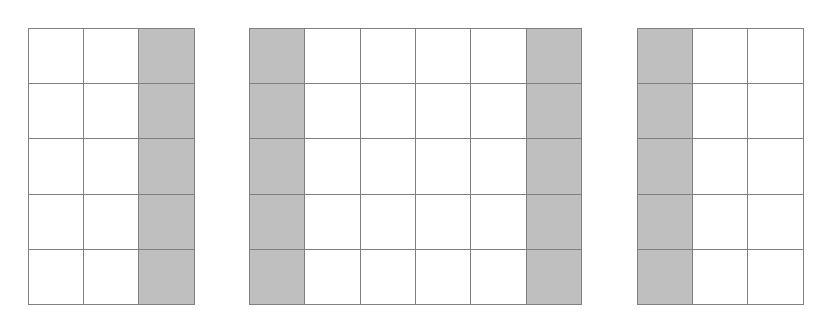
\begin{tikzpicture}[x=2em,y=2em]

  \fill[lightgray](-2,0) rectangle (-1, 5);
  \fill[lightgray] (0,0) rectangle (1,5);
  \fill[lightgray] (5,0) rectangle (6,5);
  \fill[lightgray](7,0) rectangle (8, 5);

  \drawstencil{2}{2}

  \draw[step=1, gray, very thin] (-4,0) grid (-1, 5);
  \draw[step=1, gray, very thin] (0,0) grid (6, 5);
  \draw[step=1, gray, very thin] (7,0) grid (10, 5);

\end{tikzpicture}
\end{document}

    \end{figure}
  \end{frame}

  \begin{frame}
    \frametitle{Stencil Codes - \only<1>{Decomposition}\only<2->{Boundary Exchanges}}
    \begin{figure}
      \centering
      % https://www.sharelatex.com/blog/2013/08/27/tikz-series-pt1.html

\documentclass[tikz]{standalone}
\usetikzlibrary{patterns}
\begin{document}
\newcommand{\drawstencil}[2]{%
  \draw[darkgray, thick, pattern=north west lines, pattern color=gray] (#1-1, #2) rectangle (#1+2, #2+1);
  \draw[darkgray, thick, pattern=north west lines, pattern color=gray] (#1, #2-1) rectangle (#1+1, #2+2);
  \draw[darkgray, thick, pattern=north east lines, pattern color=gray](#1, #2) rectangle (#1+1, #2+1);
}
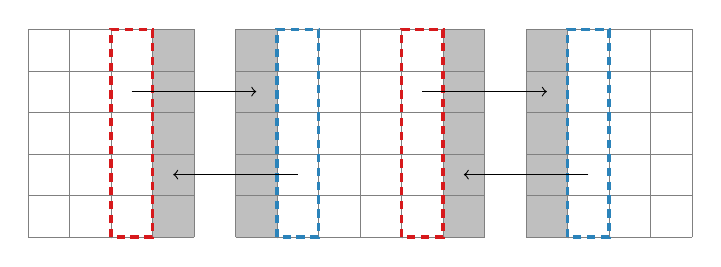
\begin{tikzpicture}[x=1.5em,y=1.5em]

  \fill[lightgray](-2,0) rectangle (-1, 5);
  \fill[lightgray] (0,0) rectangle (1,5);
  \fill[lightgray] (5,0) rectangle (6,5);
  \fill[lightgray](7,0) rectangle (8, 5);

  % Grids
  \draw[step=1, gray, very thin] (-5,0) grid (-1, 5);
  \draw[step=1, gray, very thin] (0,0) grid (6, 5);
  \draw[step=1, gray, very thin] (7,0) grid (11, 5);

  \onslide<1> {
    \drawstencil{1}{2} 
  }
  \onslide<2> {
    % Left-To-Right transmission (->)
    \draw[printred, densely dashed, very thick](-3,0) rectangle (-2, 5);
    \draw[->] (-2.5,3.5) -- (0.5,3.5);
    \draw[printred, densely dashed, very thick](4,0) rectangle (5, 5);
    \draw[->] (4.5,3.5) -- (7.5,3.5);

    % Right-To-Left transmission (<-)
    \draw[printblue, densely dashed, very thick] (1,0) rectangle (2,5);
    \draw[->] (1.5, 1.5) -- (-1.5, 1.5);
    \draw[printblue, densely dashed, very thick] (8,0) rectangle (9,5);
    \draw[->] (8.5, 1.5) -- (5.5, 1.5);
  }

\end{tikzpicture}
\end{document}

    \end{figure}
  \end{frame}

  \begin{frame}
    \frametitle{Stencil Codes}
    \begin{itemize}
      \item<1->{Memory-Centric Approach}
        \begin{itemize}
          \item{Load Neighbor Values from Memory}
          \item{Perform Calculation}
          \item{Store Result}
        \end{itemize}
      \item<2->{Not FPGA Friendly}
        \begin{itemize}
          \item{Random Access Memory Requirements}
          \item{Bi-directional data movement}
        \end{itemize}
    \end{itemize}
  \end{frame}

  \begin{frame}
    \frametitle{Stencil Codes - Communication}
    \begin{figure}
      \centering
      \documentclass[beamer]{standalone}
\definecolor{printred}{RGB}{215,25,28}
\usepackage{tikz}
\usetikzlibrary{patterns}
\begin{document}
\newcommand{\drawstencil}[2]{%
  \draw[darkgray, thick, pattern=north west lines, pattern color=gray] (#1-1, #2) rectangle (#1+2, #2+1);
  \draw[darkgray, thick, pattern=north west lines, pattern color=gray] (#1, #2-1) rectangle (#1+1, #2+2);
  \draw[darkgray, thick, pattern=north east lines, pattern color=gray](#1, #2) rectangle (#1+1, #2+1);
}
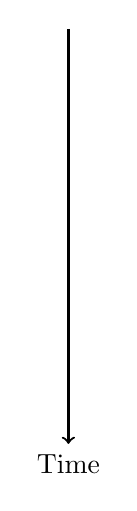
\begin{tikzpicture}[x=1.5em,y=1.5em]
  \draw[->, thick] (10,0) -- (10, -10) node (yaxis) [below] {Time};
%      \draw [<->,thick] (0,-10) node (yaxis) [above] {$y$}
%              |- (10,0) node (xaxis) [right] {$x$};
%
\end{tikzpicture}
\end{document}

    \end{figure}
  \end{frame}

  \begin{frame}
    \frametitle{Aside - Light Cones}
    \centering
    % https://www.sharelatex.com/blog/2013/08/27/tikz-series-pt1.html

\documentclass[tikz]{standalone}

\begin{document}
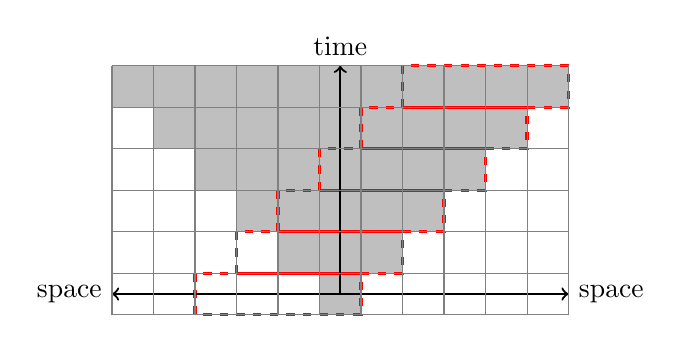
\begin{tikzpicture}[x=1.5em,y=1.5em]
  \fill[lightgray] (0,5) rectangle (11, 6);
  \fill[lightgray] (1,4) rectangle (10, 5);
  \fill[lightgray] (2,3) rectangle (9, 4);
  \fill[lightgray] (3,2) rectangle (8, 3);
  \fill[lightgray] (4,1) rectangle (7, 2);
  \fill[lightgray] (5,0) rectangle (6, 1);

  \onslide<2> {
    \foreach \ts in {0,...,5} {
      \draw[very thick, dashed, red] (\ts+2,\ts) rectangle (\ts+6,\ts+1);
     }
  }

  \draw[thick,->] (5.5,0.5) -- (5.5, 6) node (yaxis) [above] {time}; 
  \draw[thick, <->] (0,0.5) node [left] {space} -- (11,0.5) node (xaxis) [right] {space};
  \draw[gray, step=1] (0,0) grid (11,6);
\end{tikzpicture}
\end{document}

  \end{frame}

  \begin{frame}
    \frametitle{CASCADE}
  \end{frame}

  \begin{frame}
    \frametitle{Related Work}
    \begin{itemize}
      \item{Efficient temporal blocking for stencil computations by multicore-aware wavefront
      parallelization}
    \end{itemize}
  \end{frame}
\end{document}
